%%% spell check: aug 29, 2014
%%%% handouts:  pdfjam --landscape ecology2.pdf
%%%% handouts:  pdfjam --landscape --nup '2x2' ecology2.pdf

%\documentclass[handout]{beamer}
\documentclass[10pt]{beamer}
\usepackage{parskip}
\setlength{\parskip}{1.75ex}

\mode<presentation>
{\usetheme{Singapore}
\setbeamercovered{transparent}}

\title{R Minicourse Workshop, Part 2}

\author{\small Presented to the\\
        Washington State Deptment of Ecology\\
       September 2--3, 2014}

\date{\scriptsize Dr.~Robin Matthews, Institute for Watershed Studies\\
   Dr. Geoffrey Matthews, Computer Science Department\\
   Western Washington University}


\setbeamertemplate{blocks}[rounded][shadow=true]
\setbeamertemplate{footline}{\hspace*{5ex}Part 2 - Sept.~2, 2014 
   \hfill Page \insertframenumber \hspace{0.1ex} of
   \inserttotalframenumber \hspace*{5ex}
   \vspace*{2ex}}

\begin{document}
\lecture{R Minicourse}{Section 2}
\newcommand{\be}{\begin{enumerate}}
\newcommand{\ee}{\end{enumerate}}
\newcommand{\bi}{\begin{itemize}}
\newcommand{\ei}{\end{itemize}}
\newcommand{\bd}{\begin{description}}
\newcommand{\ed}{\end{description}}


\begin{frame}
\titlepage
\end{frame}

\begin{frame}
\frametitle{Graphical Presentation of Environmental Data}
\framesubtitle{How {\color{red} \em NOT} to Lie with Statistics}
\bi
\item One of the most important goals of research is to provide clear
  and unbiased summaries of the data

\item Unfortunately, it is all too easy to obscure important elements from
  research, intentionally or unintentionally

\item This portion of the {\color{red} \tt R-minicourse} will focus on
  creating effective graphical output while avoiding some of the
  more common problems

{\scriptsize
For more on data visualization:\\
{\em How to Lie with Charts} by Gerald Everett Jones (ISBN 978-1-419-65143-4)\\

\vspace{1ex}{\em Now You See It: Simple Visualization Techniques for
  Quantitative Analysis} by Stephen Few (ISBN 978-0-970-60198-8)\\

\vspace{1ex}{\em Information Dashboard Design: Displaying Data for
  At-a-Glance Monitoring} by Stephen Few (ISBN 978-1-938-37700-6)\\ }
\ei
\end{frame}




\begin{frame}
\frametitle{Principles of Scientific Visualization}
\framesubtitle{Memory Used for Processing Visual Information}

We use three basic types of memory to process
  scientific information:

\bi
\item {\color{blue} \em Iconic memory} ({\em pre-attentive
  processing}) for detecting visual information

\item {\color{blue} \em Short-term memory} ({\em attentive or
  perceptual processing}) for temporary (limited) storage and is
  limited to $\sim$3--9 items

\item {\color{blue} \em Long-term memory} for retaining information

            \bi
            {\scriptsize
            \item Long-term memory can be created consciously or unconsciously
            
            \vspace{1ex}
            \item Information is stored more permanently, with cross-links
              that allow access back into short-term memory
            
            \vspace{1ex}
            \item Required for recognizing images, interpreting words and
              numbers, understanding context\\
            }
            \ei
\ei
\end{frame}



\begin{frame}
\frametitle{Principles of Scientific Visualization}
\framesubtitle{Pre-Attentive Processing of Visual Information}

\bi 
\item {\color{blue} Iconic memory} provides quick, subconscious
  processing of graphical information and is influenced by variations
  in: 
\bi
  \item form
  \item color
  \item spatial position
  \item motion
  \ei

\item Graphics that make use of these features tend to make a strong
  impression on us, even when we don't know why

\ei

\end{frame}


\begin{frame}
\frametitle{Principles of Scientific Visualization}
\framesubtitle{Examples of Pre-Attentive Processing in Graphics}

\begin{center}
\resizebox{3.5in}{!}{
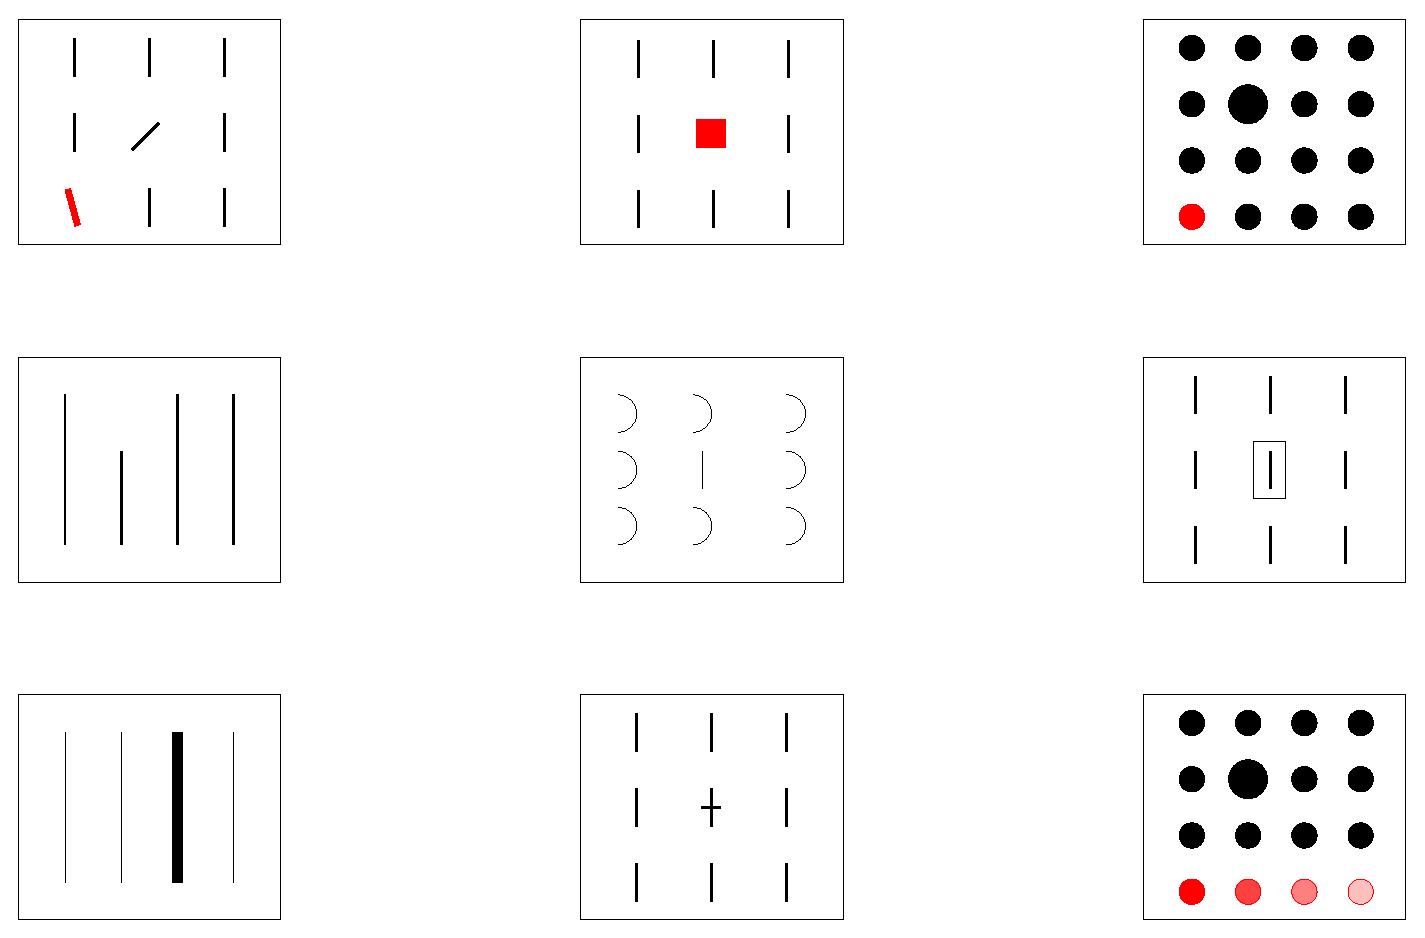
\includegraphics{./part2figures/form.eps}}
\end{center}
{\tiny Figures modified from {\color{blue} Show Me The Numbers} by Stephen Few, Analytics Press, 2004\\ }
\end{frame}


\begin{frame}
\frametitle{Principles of Scientific Visualization}
\framesubtitle{Example of Pre-Attentive Processing in Tables}

{\scriptsize
\begin{center}
\begin{tabular}{cccccccccccc}
\multicolumn{12}{c}{How many zeros are there?}\\
6     & 4    & 4    & 2    & 1    & 5    & 7    & 2    & 2    & 2    & 2    & 8    \\
9     & 8    & 9    & 3    & 6    & 5    & 5    & 5    & 7    & 8    & 7    & 6    \\
1     & 3    & 5    & 9    & 5    & 6    & 0    & 6    & 7    & 6    & 6    & 6    \\
7     & 4    & 2    & 5    & 7    & 7    & 1    & 5    & 5    & 5    & 4    & 2   \\
5     & 2    & 1    & 1    & 4    & 2    & 6    & 6    & 4    & 9    & 6    & 3    \\
5     & 7    & 2    & 0    & 6    & 1    & 6    & 8    & 0    & 6    & 0    & 2    \\
9     & 8    & 7    & 4    & 4    & 5    & 4    & 4    & 9    & 1    & 5    & 1    \\
2     & 1    & 3    & 7    & 8    & 6    & 2    & 0    & 2    & 9    & 4    & 9    \\
3     & 4    & 9    & 6    & 2    & 1    & 7    & 9    & 4    & 8    & 2    & 8    \\
2     & 5    & 5    & 2    & 2    & 4    & 5    & 5    & 8    & 7    & 1    & 5    \\
\end{tabular}
\end{center}
}

{\scriptsize
\begin{center}
\begin{tabular}{cccccccccccc}
\multicolumn{12}{c}{How many zeros are there?}\\
6     & 4    & 4    & 2    & 1    & 5    & 7    & 2    & 2    & 2    & 2    & 8    \\
9     & 8    & 9    & 3    & 6    & 5    & 5    & 5    & 7    & 8    & 7    & 6    \\
1     & 3    & 5    & 9    & 5    & 6    & {\bf \small \color{red}0}    & 6    & 7    & 6    & 6    & 6    \\
7     & 4    & 2    & 5    & 7    & 7    & 1    & 5    & 5    & 5    & 4    & 2   \\
5     & 2    & 1    & 1    & 4    & 2    & 6    & 6    & 4    & 9    & 6    & 3    \\
5     & 7    & 2    & {\bf \small \color{red}0}    & 6    & 1    & 6    & 8    & {\bf
  \small \color{red}0}    & 6    & {\bf \small \color{red}0}    & 2    \\
9     & 8    & 7    & 4    & 4    & 5    & 4    & 4    & 9    & 1    & 5    & 1    \\
2     & 1    & 3    & 7    & 8    & 6    & 2    & {\bf \small \color{red}0}    & 2    & 9    & 4    & 9    \\
3     & 4    & 9    & 6    & 2    & 1    & 7    & 9    & 4    & 8    & 2    & 8    \\
2     & 5    & 5    & 2    & 2    & 4    & 5    & 5    & 8    & 7    & 1    & 5    \\
\end{tabular}
\end{center}
}

\end{frame}


\begin{frame}
\frametitle{Principles of Scientific Visualization}
\framesubtitle{Perceptual Processing of Visual Information}

\bi 
\item {\color{blue} Short-term} and {\color{blue} long-term
  memory} require conscious interpretation of visual information

\item As a result, it is easy to fool our visual perception of data,
  especially if you use pre-attentive processing

\item In creating scientific graphics, careful use
  of color, shape, and position can {\large \bf \color{red}
  emphasize} or {\tiny \color{yellow} de-emphasize} information

\item Two major objectives in designing good tables or figures:

\bi
\item Highlight the data by enhancing ``data ink'' (reduce non-data ink)
\item Organize the data by grouping, prioritizing, and sequencing
\ei
\ei

\end{frame}


\begin{frame}
\frametitle{Principles of Scientific Visualization}
\framesubtitle{Perceptual Processing of Visual Information}

\bi 
\item Short-term and long-term memory involves
  conscious interpretation of visual information

\item As a result, it is easy to fool our visual perception of data,
  especially if you use pre-attentive processing

\item In creating scientific graphics, careful use of color, shape,
  and position can emphasize or de-emphasize information

\item {\color{red} Two major objectives} in designing good tables or
  figures:

\bi
\item {\color{blue} Highlight the data} by enhancing ``data ink''
  (reduce non-data ink)
\item {\color{blue} Organize the data} by grouping, prioritizing, and sequencing
\ei
\ei

\end{frame}


\begin{frame}[fragile]
\frametitle{Building Simple Scatterplots Using {\color{red} \tt plot()}}
\label{figTP1}
\vspace*{2ex}
{\scriptsize
One of the most versatile plotting tools in {\color{red} \tt R}
  is the {\color{red} \tt plot()} function. In its simplest form, it
  can be used with very little modification to explore the data\\
If necessary, re-enter {\color{red} \tt read.table("lakes.csv", T, sep=","); attach(lakes)}
}

\vspace*{-4ex}
\begin{center}
\resizebox{3in}{!}{
\includegraphics{./part2figures/tp1.ps}}
\end{center}
\end{frame}


\begin{frame}[fragile]
\frametitle{Plotting One Variable Using Points, Lines, or Both}
\label{figTP2}
\vspace*{-2ex}
\begin{center}
\resizebox{3.5in}{!}{
\includegraphics{./part2figures/tp2.ps}}
\end{center}
\end{frame}


\begin{frame}[fragile]
\frametitle{Changing Colors, Characters, Lines}
\label{figTP3}
\vspace*{-2ex}
\begin{center}
\resizebox{3.5in}{!}{
\includegraphics{./part2figures/tp3.ps}}
\end{center}
\end{frame}


\begin{frame}[fragile]
\frametitle{Saving and Copying {\color{red} \tt R} Figures}

{\small
\bi
\item {\color{red} \tt R} figures are directed to the graphics
  window

\item Individual figures can be saved or copied from this window -
  select ``emf'' to minimize pixelation

\item Each new figure overwrites the previous one unless you direct
  {\color{red} \tt R} to pause between figures:

{\scriptsize \color{red}
\verb%par(ask=T)  ### graphics window freezes between plots%\\
\verb%            ### hit any key to see next figure%\\
\verb%par(ask=F)  ### unfreezes graphics window%\\
}

\item A better approach is to save the output using a source file

{\scriptsize
$\Rightarrow$This would be a good time to use source files
({\color{red} \tt R-minicourse}, Part 1)\\}

\item The syntax for saving graphical output varies slightly for
  different operating systems; use {\color{red}
    \tt savePlot} for Windows:

{\scriptsize \color{red}
\verb%plot(tp, chl)%\\
\verb%savePlot(filename = "simpleplot", type="emf")%\\
\verb%### type="pdf" also produces nice figures%\\
}
\ei 
}
\end{frame}


\begin{frame}[fragile]
\frametitle{Plotting One Variable vs.~Time}

\vspace{2ex} 

{\scriptsize We usually want an informative x-axis rather than the row
  number (Index).  It is very simple to add month (column 2) and year
  (column 4)\\}

\vspace*{-1ex}
\begin{center}
\resizebox{3in}{!}{
\includegraphics{./part2figures/tp4.ps}}
\end{center}
\end{frame}


\begin{frame}[fragile]
\frametitle{Plotting Time Using the {\color{red} \tt chron} Library}

\bi
\item One of the most powerful features of {\color{red} \tt R} is
  that it is open-source and programmable, so individuals can
  contribute {\em libraries} or {\em packages} containing specialized
  programs

\item The {\color{red} \tt chron} library is designed to recognize
  time in a variety of formats, and is easily integrated with other
  functions like {\color{red} \tt plot()}

\item $\Rightarrow$The {\color{red} \tt chron} may need to be
  installed on your computer.  Click on ``install package'' at the top
  of the R window, select USA (WA1) as the mirror\footnote{\scriptsize
    Mirrors are sites that maintain exact copies of R libraries.\\},
  then scroll down until you find {\color{red} \tt chron}.  It should
  install automatically

\item Before you can use the library you need to tell {\color{red} \tt
  R} to read the library:

{\scriptsize \color{red} 
\verb%library(chron) ### this will load chron during your work session%\\
\verb%library()      ### this lists all active libraries%\\
}

\ei
\end{frame}

\begin{frame}[fragile]
\frametitle{Using the {\color{red} \tt chron} Library, continued}

\bi
\item The IWS policy is to keep month, day, year ($\pm$time) in
  separate columns to minimize spreadsheet date conversion errors

\item But {\color{red} \tt chron} expects the date to be in typical
  spreadsheet format (month/day/year and hour:min:sec), so we use a
  function to paste the columns together:

{\scriptsize \color{red}
\verb%mdy.chron <- function(month, day, year) {%\\
\verb%  chron(dates.=paste(month, day, year, sep="/"))%\\
\verb%}%\\
}

\item Now we can use {\color{red} \tt mdy.chron(month, day, year)} as
  a variable for the x-axis (see top figure on page \pageref{chronfig})

{\scriptsize \color{red}
\verb%plot(tp ~ mdy.chron(month, day, year))%\\
}
\ei
\end{frame}

\begin{frame}[fragile]
\frametitle{Using the {\color{red} \tt chron} Library, continued}

Here is a more advanced example (see bottom figure on page
\pageref{chronfig})

{\scriptsize \color{red}
\verb%### create a "nice" date range for the x-axis%\\
\verb%xdates <- c(mdy.chron(1,1,2007), mdy.chron(12, 31, 2013))%\\

\vspace{2ex}
\verb%### plot the data, with x/y axis labels and annotations%\\
\verb%plot(tp ~ mdy.chron(month, day, year),%\\
\verb%     xlim=xdates,%\\
\verb%     xlab=" ",%\\
\verb%     ylim=c(0, 1000),%\\
\verb%     ylab="TP (ug-P/L)",%\\
\verb%     pch=21, bg="skyblue", cex=1.5)%\\

\vspace{2ex}
\verb%### add a text line to identify the outlier%\\
\verb%text(x=mdy.chron(6,28,2010), y=850, "Wiser Lake, June 28, 2010",%\\
\verb%     cex=0.75, col="red")%\\
}

\end{frame}


\begin{frame}[fragile]
\label{chronfig}
\begin{center}
\resizebox{3in}{!}{
\includegraphics{./part2figures/tp5.ps}}
\end{center}
\end{frame}

\begin{frame}[fragile]
\frametitle{Plotting Two Variables Using {\color{red} \tt plot()}}
\vspace*{-3ex}
\begin{center}
\resizebox{3.5in}{!}{
\includegraphics{./part2figures/tp6.ps}}
\end{center}
\end{frame}


\begin{frame}[fragile]
\frametitle{Advanced Scatterplot Features}
\framesubtitle{Legends, Text, Expressions, Polygons}
\label{advancedscatterplots}
{\color{red} \scriptsize

\begin{verbatim}
### Step #1: create an empty plot (type="n"); 
###          this will let us place the polygon layer beneath the data
plot(log10(chl), log10(tp), type="n",
     xlab=expression(paste("Chl"[log10] ~ (mu * "g/L"))),
     ylab=expression(paste("TP"[log10] ~ (mu * "g-P/L"))))

### Step #2: draw a shaded, borderless rectangle showing tp detection limit
rect(xleft=-1.1, ybottom=-0.5, xright=2.9, ytop=log10(2), col="pink", border=NA)

### Step #3: add the chlorophyll and total phosphorus data using points
points(log10(chl), log10(tp),
     pch=21, bg="skyblue", cex=1.5)

### Step #4: add a horizontal line at the tp "action" level (20 ug/L)
abline(h=log10(20), lty=2, lwd=2, col="red")

### Step #5: use text and legend to annotate the figure;
###          paste and expression are used to add math symbols and subscripts
text(x=2.5, y=0.25, "TP detection limit", cex=0.7, col="red")
legend(x="topleft", expression("20" * ~ mu * "g-P/L"),
       lty=2, lwd=2, col="red", bty="n")
\end{verbatim}
}
\end{frame}


\begin{frame}[fragile]
\begin{center}
\resizebox{3in}{!}{
\includegraphics{./part2figures/tp7.ps}}
\end{center}
\end{frame}



\begin{frame}[fragile]
\frametitle{Summary of Scatterplot Syntax}
\label{scatterplotsyntax}

{\scriptsize
\begin{center}
\begin{tabular}{ll}\hline
\multicolumn{2}{l}{Basic plotting syntax}\\
{\color{red} \tt plot(x,y)} or {\color{red} \tt plot(y$\sim$x)} 
           & Plot x (horizontal) and y (vertical)\\
           & type=points (p), lines (l), both (b), overplot (o)\\
{\color{red} \tt points(x,y)}, {\color{red} \tt lines(x, y)}
           & Can be used for scatterplots; adds points/lines to existing plot\\
{\color{red} \tt xlim}, {\color{red} \tt ylim}
        & set x- or y-limits (e.g., xlim=c(0, 100))\\
{\color{red} \tt lty}, {\color{red} \tt lwd} & Sets line type and line width\\
           & \\
\multicolumn{2}{l}{Syntax for annotating scatterplots}\\
{\color{red} \tt cex}
        & character expansion; subgroups can be specified (e.g., cex.axis)\\
{\color{red} \tt col}, {\color{red} \tt bg} 
        & Sets color; subgroups can be specified (e.g., col.axis);\\
        & {\color{red} \tt bg} used for pch 21-25 \\
        & {\color{red} \tt col=NA} is transparent\\
{\color{red} \tt pch} & Plotting characters (1-16 regular; 21-25 dual color)\\
{\color{red} \tt xlab}, {\color{red} \tt ylab}, {\color{red} \tt main} 
        & Adds main, x- or y-axis labels; can include spaces, etc\\
                 & \\
\multicolumn{2}{l}{Misc}\\
{\color{red} \tt abline} & Add lines to existing plot; 
        modify with {\color{red} \tt lty}, {\color{red} \tt lwd}\\
                 & \hspace{2ex} h or v = numerical value (horizontal/vertical lines)\\
                 & \hspace{2ex} a, b = intercept and slope (0,1 for 1:1 diagonal)\\
                 & \hspace{2ex} {\color{red} \tt lm} object (regression line)\\
{\color{red} \tt rect}, {\color{red} \tt polygon}, {\color{red} \tt segments}
                & Add rectangles, polygons, line segments to existing plot\\
 {\color{red} \tt legend}, {\color{red} \tt text}
                & Add legends or text to existing plot\\ \hline
\multicolumn{2}{l}{{\color{red} \tt ?par}, {\color{red} \tt ?plot},
  {\color{red} \tt legend}, etc.~will bring up help screen}\\
\end{tabular}



\end{center}
}
\end{frame}


\begin{frame}[fragile]
\frametitle{Plotting Examples Using Iris Data}
\begin{center}
\resizebox{3in}{!}{
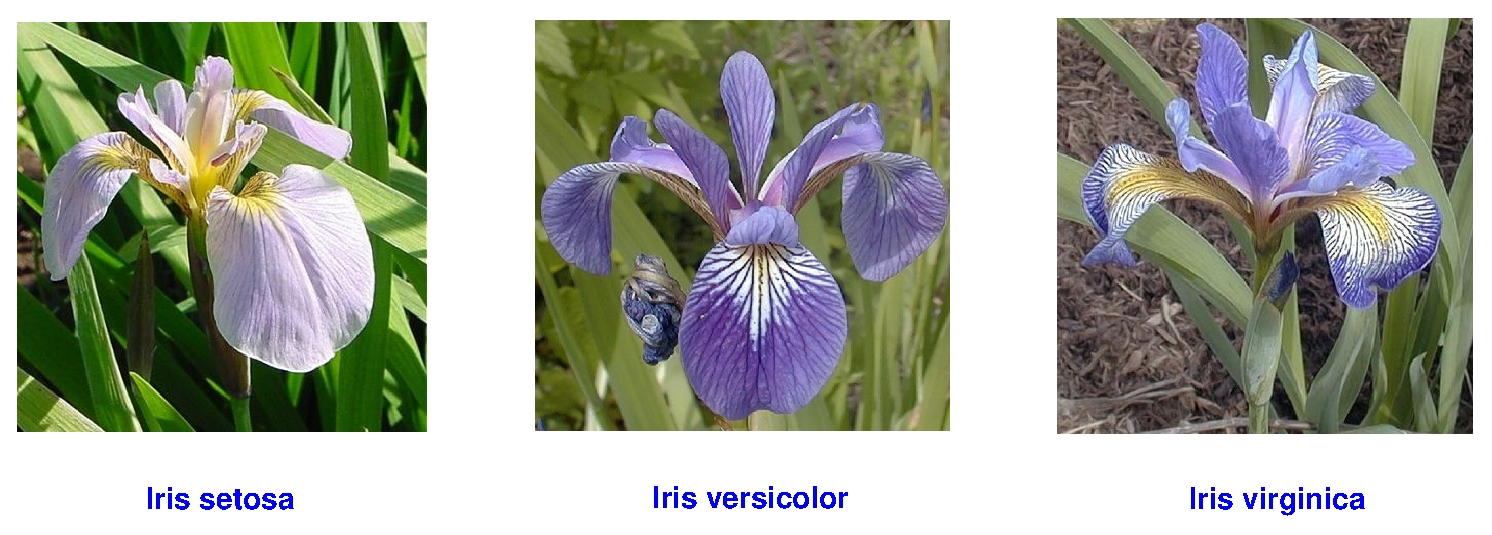
\includegraphics{./part2figures/irises.eps}}
\end{center}

\bi
{\scriptsize
\item Boxplots are an excellent exploratory tool
  for summarizing {\em categorical} groups of data

\item We will use Fisher's Iris data to illustrate scatterplot
  techniques

\item The iris data consist of sepal and petal width and length
  measurements collected from 150 iris flowers representing three
  species of iris (n=50 for each species; species={\em Iris setosa},
  {\em Iris versicolor}, and {\em Iris virginica})
\item These data were first published by R.A. Fisher in ``The use of
  multiple measurements in taxonomic problems'' (Annals of Eugenics
  7:179-188, 1936)
\item The iris data are included with the R base library and can be
  loaded and attached using {\tt \color{red} data(iris);
    attach(iris)}\\} \ei

{\tiny Photographs by C.~Hensler and D.~Kramb; used with permission}

\end{frame}

\begin{frame}
\begin{center}
\resizebox{3in}{!}{
	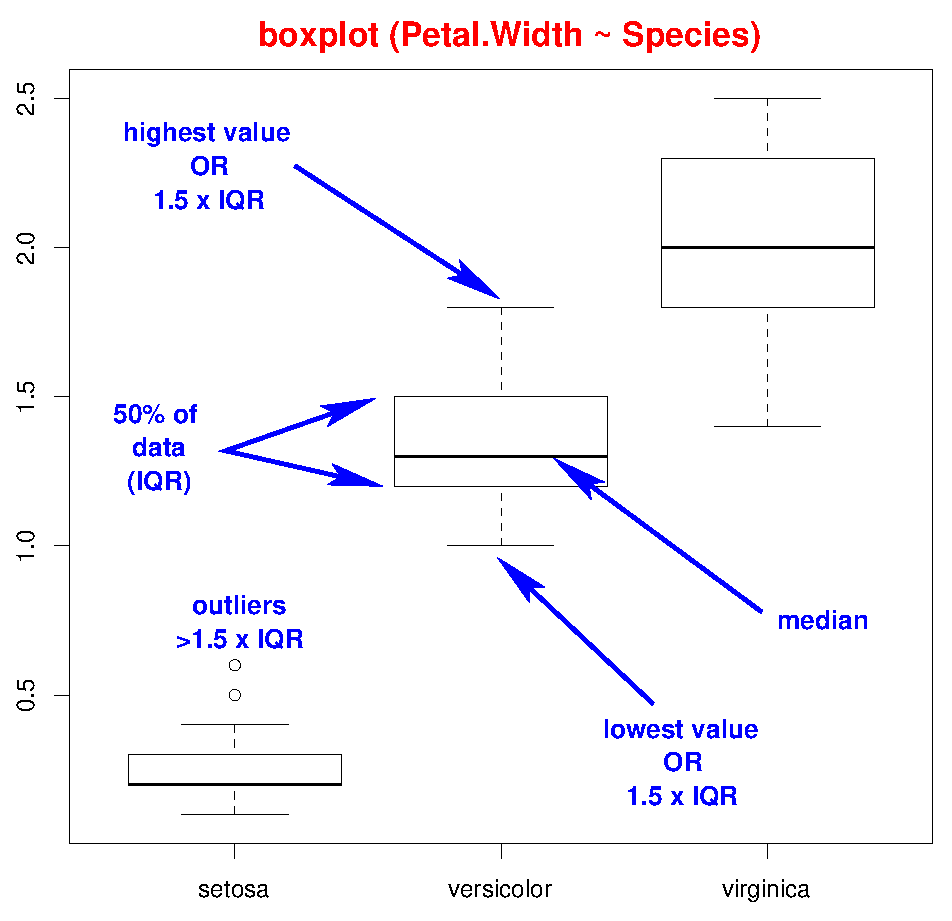
\includegraphics{./part2figures/irisboxplot1.eps}}
\end{center}
\end{frame}




\begin{frame}[fragile]
\frametitle{Annotated Boxplots of the Iris Data}

\bi

\item Many of the commands you learned for scatterplots will also work
  with boxplots

\item This code produces notched, annotated boxplots (page
  \pageref{notchedboxplot}) that shows intervals of significance:

\[
{\rm median} \pm 1.58 \times \frac{\rm IQR}{\sqrt{n}}
\]


If the notches overlap, the medians are not significantly different

{\scriptsize
\color{red}
\begin{verbatim}
boxplot(Sepal.Width ~ Species, 
   ylab="Sepal Width (cm)", main="Boxplot of Iris Sepal Width",
   notch = T, boxwex = 0.5,
   col = c("mistyrose", "skyblue", "orchid"),
   border=c("hotpink4", "skyblue4", "mediumorchid4"),
   names = c("Iris setosa", "Iris versicolor", "Iris virginica"))

### want a list of all colors? type colors()
\end{verbatim}
}

\ei

\end{frame}



\begin{frame}
\label{notchedboxplot}
\begin{center}
\resizebox{3in}{!}{
	\includegraphics{./part2figures/irisboxplot2.ps}}
\end{center}
\end{frame}


\begin{frame}
\frametitle{Requesting Boxplots Summary Statistics}

You can request the plotting
  statistics, including notch intervals, by adding
  {\color{red} \tt plot=F} in the boxplot syntax


\begin{center}
\resizebox{2.75in}{!}{
	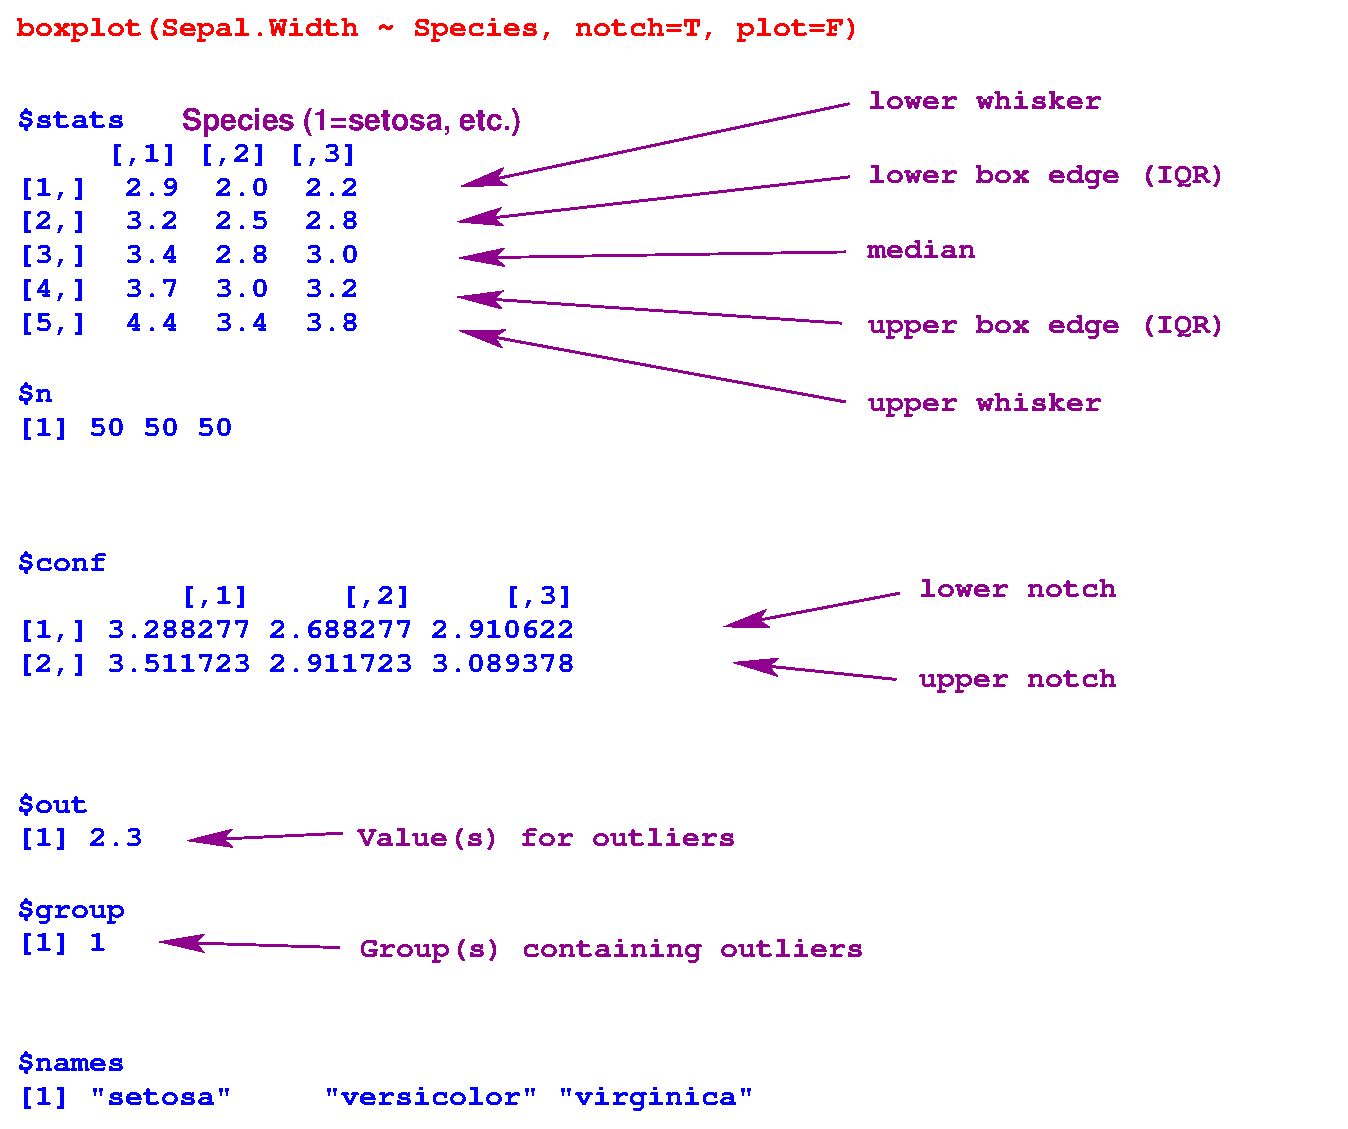
\includegraphics{./part2figures/boxplotstats.eps}}
\end{center}
\end{frame}


\begin{frame}[fragile]
\frametitle{Adding Legends to Simple Boxplots}

Here is how to use {\color{red} \tt legend} to identify
  categorical groups:

{\scriptsize \color{red}
\verb%legend(x="topleft", c("Iris setosa", "Iris versicolor", "Iris virginica"),%\\
\verb%   fill=c("pink", "violet", "purple"), bty="n")%\\
}


\vspace*{-2ex}
\begin{center}
\resizebox{2.5in}{!}{
	\includegraphics{./part2figures/irisboxplot4.ps}}
\end{center}

\end{frame}



\begin{frame}[fragile]
\frametitle{Paired Boxplots Using Guinea Pig Data}

\bi
\item You can used paired boxplots to plot more than one type of categorical data on the x-axis

\item This example uses guinea pig tooth growth data receiving three
  doses of Vitamin C (0.5, 1, and 2 mg) from either orange juice or
  ascorbic acid

{\scriptsize \color{red}
\verb%data(ToothGrowth) #data included with R base library%\\
\verb%attach(ToothGrowth)%\\
\verb%summary(ToothGrowth)%\\

\vspace{2ex}
\color{blue}
\verb%      len        supp         dose%\\
\verb% Min.   : 4.20   OJ:30   Min.   :0.500%\\
\verb% 1st Qu.:13.07   VC:30   1st Qu.:0.500%\\
\verb% Median :19.25           Median :1.000%\\
\verb% Mean   :18.81           Mean   :1.167%\\
\verb% 3rd Qu.:25.27           3rd Qu.:2.000%\\
\verb% Max.   :33.90           Max.   :2.000%\\
}
\ei
\end{frame}



\begin{frame}[fragile]
\frametitle{Paired Boxplots - Annotated {\color{red} \tt R} Syntax}

{\scriptsize \color{red}
\verb%boxplot(len ~ dose,%\\
\verb%     boxwex = 0.25, at = 1:3 - 0.2,%\\
\verb%     subset = supp == "VC", col = "lightyellow",%\\
\verb%     xlab = "Vitamin C dose (mg)",%\\
\verb%     ylab = "Tooth Length (mm?)", ylim = c(0, 35), yaxs = "i")%\\

\vspace{1ex}
\color{blue}
\verb%### the first plot sets up the template, including axis and main lagels%\\
\verb%### yaxs = "i" helps create better axis intervals%\\

\verb%### "at" lists the number of primary categories (1:3) for vitamin C doses%\\
\verb%### and adds location (-0.2) to offset each box slightly left of center%\\

\verb%### "subset" selects the ascorbic acid group (VC)%\\

\vspace{3ex}
\color{red}
\verb%boxplot(len ~ dose, add = TRUE,%\\
\verb%     boxwex = 0.25, at = 1:3 + 0.2,%\\
\verb%     subset = supp == "OJ", col = "darkorange")%\\

\vspace{1ex}
\color{blue}
\verb%### "add=TRUE" will add the second plot to the same figure%\\
\verb%### "at" matchs previous but offsets boxes in opposite direction%\\


\vspace{3ex}
\color{red}
\verb%legend(x="bottomright", c("Ascorbic acid", "Orange juice"),%\\
\verb%     fill = c("lightyellow", "darkorange"))%\\

\vspace{1ex}
\color{blue}
\verb%### note that default legend outline was NOT removed%\\
}
\end{frame}



\begin{frame}
\begin{center}
\resizebox{3in}{!}{
	\includegraphics{./part2figures/toothgrowth1.ps}}
\end{center}
\end{frame}

\begin{frame}
\begin{center}
\resizebox{3in}{!}{
	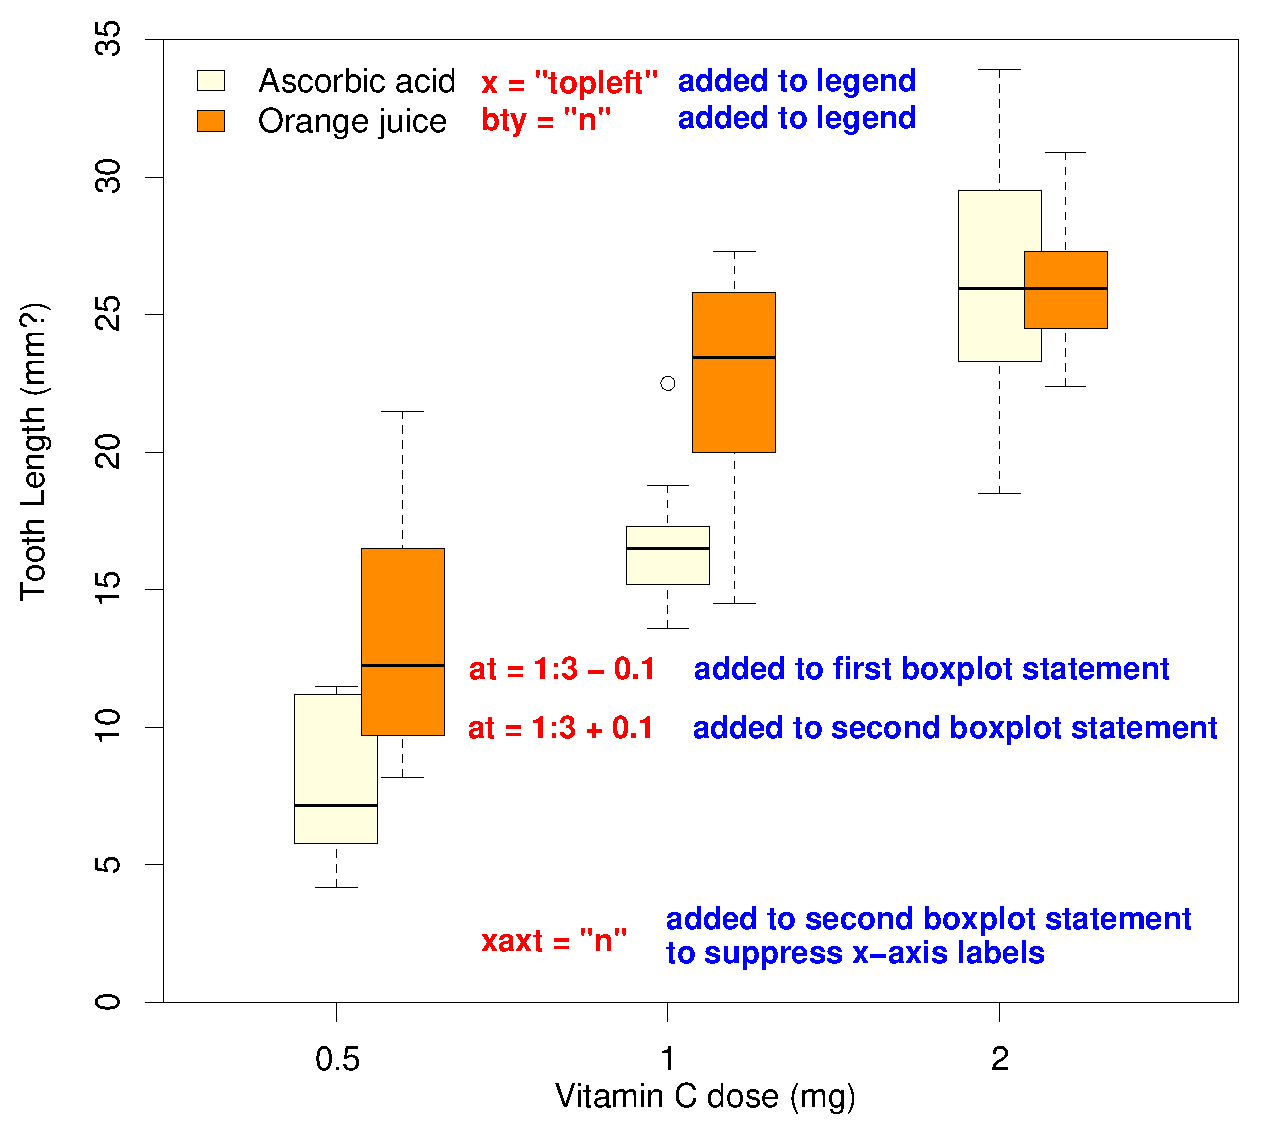
\includegraphics{./part2figures/toothgrowth2.eps}}
\end{center}
\end{frame}


\begin{frame}[fragile]
\frametitle{Advanced Boxplot Features}
\framesubtitle{Adding Raw Data to Boxplots using {\color{red} \tt points()} and {\color{red} \tt jitter()}}
\label{advancedscatterplots}
{\color{red} \footnotesize
\verb%with(ToothGrowth,%\\
\verb%     {%\\
\verb%      boxplot(len~supp, border=c("darkorange3", "gold4"),%\\
\verb%              col=c("darkorange", "gold"), boxwex=0.5,%\\
\verb%              ylab="Tooth Growth",%\\
\verb%              names=c("Orange Juice", "Vitamin C"))%\\

\vspace{1ex}
\color{blue}
\verb%### "with" defines the data set; the rest is basic boxplot syntax%\\

\color{red}
\vspace{3ex}
\verb%      points(jitter(rep(1:2, each=30), 0.5),%\\
\verb%             unlist(split(len, supp)),%\\
\verb%             cex=1.25, pch=16, %\\
\verb%             col=c("gold4", "darkorange3")[unclass(ToothGrowth$supp)])%\\
\verb%     })%\\

\vspace{1ex}
\color{blue}
\verb%### "points" is similar to previous scatterplot examples %\\
\verb%### "jitter" prevents points from plotting on top of each other %\\
\verb%###  with 30 points in each group centered on boxes 1-2) %\\
\verb%### "unlist(split) puts the tooth length data into "supp" groups %\\
\verb%### "unclass" is used to assign correct colors based on "supp" groups %\\
}
\end{frame}


\begin{frame}[fragile]
\frametitle{Boxplot With Jittered Data Points}
\begin{center}
\resizebox{3in}{!}{
\includegraphics{./part2figures/toothgrowth3.ps}}
\end{center}
\end{frame}



\begin{frame}[fragile]
\frametitle{Summary of Boxplot Syntax}

{\footnotesize
\begin{tabular}{ll}
Syntax                    & Description \\ \hline
\multicolumn{2}{l}{Syntax for changing widths}\\
{\color{red} \tt boxwex}  & Set scale for all boxes; values $<$1 make boxes narrower\\
{\color{red} \tt staplewex} & Set scale width of staple line; proportional to box width\\
{\color{red} \tt outwex}  & Set scale width of outlier line; proportional to box width \\
                          & \\
\multicolumn{2}{l}{Syntax for changing colors}\\
{\color{red} \tt border}  & Use to add colors to the box borders (see iris examples)\\
{\color{red} \tt col}     & Use to add colors to the boxes (see iris examples) \\
                          & \\
\multicolumn{2}{l}{Syntax for adding features}\\
{\color{red} \tt names}   & Use to add group labels (see iris examples)\\
{\color{red} \tt notch}   & {\color{red} \tt notch=T} will add notches\\
{\color{red} \tt range}   & Defines range for boxplot whiskers; default=1.5 $\times$box width;\\
                          & {\color{red} \tt range=0} will extend whiskers to max/min values\\ 
                          & \\
\multicolumn{2}{l}{Misc}\\
{\color{red} \tt add}     & {\color{red} \tt add=TRUE} will add boxplot to current plot\\
{\color{red} \tt at}      & Box locations; when {\color{red} \tt add=TRUE},
                            {\color{red} \tt at} = 1:n (n=number of boxes)\\
{\color{red} \tt plot}    & {\color{red} \tt plot=F} suppresses plotting, but lists statistics\\\hline
\end{tabular}

Also see scatterplot syntax (page \pageref{scatterplotsyntax})

}

\end{frame}

\begin{frame}
\frametitle{Supplemental References}

\bi
\item Lander, Jared P.  2014.  R for Everyone, Advanced Analytics and
  Graphics.  Addison Wesley Data \& Analytics Series, ISBN
  978-0-321-88803-7.

\item Murrell, Paul.  2011.  R Graphics, CRC Press.  ISBN
  978-1-4398-3176-2.

\item Teetor, Paul. 2011.  The R Cookbook.  O'Reilly Publishers. ISBN
  978-0-596-880915-7.

\item Wickham, Hadley.  2009.  ggplot2: Elegant Graphics for Data
  Analysis (UseR!).  Springer.  ISBN 978-0-387-98140-6.
\ei
\end{frame}



\end{document}
\end
